\section{Рабочий проект}
\subsection{Модули программной системы}
\subsubsection{Модуль app.py}
Модуль представляет собой серверную часть приложения. Реализован с использованием фреймворка Flask. Отвечает за обработку HTTP-запросов, взаимодействие с базой данных PostgreSQL, управление заказами, книгами, авторами, жанрами, тегами и пользователями. Внутренние
поля представлены в таблице 4.1.

% Таблица для app.py
\begin{xltabular}{\textwidth}{|p{4.5cm}|>{\setlength{\baselineskip}{0.7\baselineskip}}p{4.5cm}|>{\setlength{\baselineskip}{0.7\baselineskip}}X|}
	\caption{Внутренние поля модуля app.py\label{table:app.py_fields}}\\
	\hline \centrow \setlength{\baselineskip}{0.7\baselineskip} Внутреннее поле & \centrow \setlength{\baselineskip}{0.7\baselineskip} Тип поля & \centrow Описание поля \\ \hline
	\endfirsthead
	\caption*{Продолжение таблицы \ref{table:app.py_fields}}\\ 
	\centrow Внутреннее поле & \centrow Тип поля & \centrow Описание поля \\ \hline
	\finishhead
	app & Flask & Экземпляр приложения Flask, используемый для маршрутизации и обработки запросов \\ \hline
\end{xltabular}

Методы модуля представлены в таблице 4.2.
% Таблица для app.py
\begin{xltabular}{\textwidth}{|>{\raggedright\arraybackslash}X|>{\raggedright\arraybackslash}X|>{\raggedright\arraybackslash\setlength{\baselineskip}{0.7\baselineskip}}X|>{\raggedright\arraybackslash\setlength{\baselineskip}{0.7\baselineskip}}X|}
	\caption{Методы модуля app.py\label{table:app.py}}\\
	\hline \centrow \setlength{\baselineskip}{0.7\baselineskip} Название метода & \centrow \setlength{\baselineskip}{0.7\baselineskip} Параметры метода & \centrow Возвращаемое значение & \centrow Описание метода \\ \hline
	\endfirsthead
	\caption*{Продолжение таблицы \ref{table:app.py}}\\ 
	\hline \centrow \setlength{\baselineskip}{0.7\baselineskip} Название метода & \centrow \setlength{\baselineskip}{0.7\baselineskip} Параметры метода & \centrow Возвращаемое значение & \centrow Описание метода \\ \hline
	\finishhead
	default & obj: Any — объект для сериализации & Сериализуемый объект (float для Decimal, str для date/datetime, или результат базового метода) & Преобразует объекты типа Decimal в float, date/datetime в строку ISO-формата, для остальных вызывает базовый метод JSONEncoder \\ \hline
	get\_db & Отсутствуют & psycopg2.connect — объект соединения с базой данных & Устанавливает соединение с базой данных PostgreSQL (bookstore\_db) \\ \hline
	json\_response & data: Any — данные для ответа, status: int (по умолчанию 200) — HTTP-код статуса & Response — объект HTTP-ответа с MIME-типом application/json & Формирует JSON-ответ с использованием Custom JSONEncoder \\ \hline
	create\_order & Отсутствуют (данные из HTTP POST-запроса: user\_id, items, total\_amount) & JSON-ответ с информацией о заказе или ошибкой & Создает заказ, проверяет наличие книг на складе, обновляет склад, добавляет элементы заказа \\ \hline
	get\_user\_orders & user\_id: int — идентификатор пользователя & JSON-ответ со списком заказов или ошибкой & Получает список заказов пользователя с деталями о книгах, отсортированных по дате \\ \hline
	update\_order\_ status & order\_id: int — ID заказа, JSON-данные с полем status & JSON-ответ с подтверждением или ошибкой & Обновляет статус заказа, проверяет валидность статуса \\ \hline
	get\_all\_orders & Отсутствуют & JSON-ответ со списком всех заказов или ошибкой & Получает все заказы с информацией о пользователях и книгах \\ \hline
	get\_books & Параметры запроса: search: str — поисковый запрос, page: int — номер страницы, per\_page: int — книг на странице & JSON-ответ с книгами и данными пагинации & Получает список книг с поддержкой поиска и пагинации \\ \hline
	get\_book & book\_id: int — ID книги & JSON-ответ с данными книги или ошибкой & Получает детальную информацию о книге, включая жанры и автора \\ \hline
	create\_book & JSON-данные: title, author\_id, price, quantity\_in\_stock, description, publication\_date, cover\_image\_url, genres, tags & JSON-ответ с ID новой книги или ошибкой & Создает новую книгу и связывает её с жанрами и тегами \\ \hline
	delete\_book & book\_id: int — ID книги & JSON-ответ с подтверждением или ошибкой & Удаляет книгу из базы данных \\ \hline
	get\_authors & Отсутствуют & JSON-ответ со списком авторов или ошибкой & Получает список всех авторов \\ \hline
	search\_authors & name: str — поисковый запрос по имени автора & JSON-ответ со списком авторов или ошибкой & Выполняет поиск авторов по имени (ограничение 10 результатов) \\ \hline
	create\_author & JSON-данные: name: str — имя автора & JSON-ответ с ID нового автора или ошибкой & Создает нового автора в базе данных \\ \hline
	get\_genres & Отсутствуют & JSON-ответ со списком жанров или ошибкой & Получает список всех жанров \\ \hline
	get\_tags & Отсутствуют & JSON-ответ со списком тегов или ошибкой & Получает список всех тегов \\ \hline
	get\_cart\_books & ids: str — строка с ID книг, разделённых запятыми & JSON-ответ со списком книг или ошибкой & Получает информацию о книгах в корзине по их ID \\ \hline
	register & JSON-данные: username: str, password: str, email: str & JSON-ответ с данными пользователя или ошибкой & Регистрирует нового пользователя с ролью customer \\ \hline
	login & JSON-данные: username: str, password: str & JSON-ответ с данными пользователя или ошибкой & Аутентифицирует пользователя по имени и паролю \\ \hline
	update\_book & book\_id: int, JSON-данные: title, author\_id, price, quantity\_in\_stock, description, publication\_date, cover\_image\_url, genres, tags & JSON-ответ с подтверждением или ошибкой & Обновляет данные книги, включая жанры и теги \\ \hline
	update\_role & JSON-данные: username: str, new\_role: str & JSON-ответ с данными пользователя или ошибкой & Обновляет роль пользователя, проверяет валидность роли \\ \hline
	get\_users & Отсутствуют & JSON-ответ со списком пользователей или ошибкой & Получает список всех пользователей с их ролями \\ \hline
\end{xltabular}

\subsubsection{Модуль app.js}

Модуль app.js — клиентская часть приложения, реализованная на JavaScript. Отвечает за взаимодействие с сервером через API, управление корзиной, отображение книг, заказов, управление пользователями и администраторскими функциями. Внутренние поля представлены в таблице 4.3.
% Таблица для app.js
\begin{xltabular}{\textwidth}{|p{4.5cm}|>{\setlength{\baselineskip}{0.7\baselineskip}}p{4.5cm}|>{\setlength{\baselineskip}{0.7\baselineskip}}X|}
	\caption{Внутренние поля модуля app.js\label{table:app.js_fields}}\\
	\hline \centrow \setlength{\baselineskip}{0.7\baselineskip} Внутреннее поле & \centrow \setlength{\baselineskip}{0.7\baselineskip} Тип поля & \centrow Описание поля \\ \hline
	\endfirsthead
	\caption*{Продолжение таблицы \ref{table:app.js_fields}}\\ 
	\hline \centrow \setlength{\baselineskip}{0.7\baselineskip} Внутреннее поле & \centrow \setlength{\baselineskip}{0.7\baselineskip} Тип поля & \centrow Описание поля \\ \hline
	\finishhead
	cart & Array & Локальная корзина пользователя, хранящая ID книг и их количество, сохраняется в localStorage \\ \hline
	allBooks & Array & Список всех книг, полученных с сервера, используется для отображения и управления \\ \hline
	cartBooks & Array & Список книг в корзине с полной информацией, полученной с сервера \\ \hline
	cartEventInitialized & Boolean & Флаг, указывающий, инициализированы ли обработчики событий корзины \\ \hline
	currentUser & Object или null & Объект текущего авторизованного пользователя, хранится в localStorage \\ \hline
	currentPage & Number & Текущая страница пагинации для списка книг \\ \hline
	booksPerPage & Number & Количество книг, отображаемых на одной странице (по умолчанию 8) \\ \hline
	authDropdownVisible & Boolean & Флаг, указывающий, отображается ли выпадающее меню аутентификации \\ \hline
	ordersDropdownVisible & Boolean & Флаг, указывающий, отображается ли выпадающее меню заказов \\ \hline
\end{xltabular}

Методы модуля представлены в таблице 4.4.
% Таблица для app.js
\begin{xltabular}{\textwidth}{|>{\raggedright\arraybackslash}X|>{\raggedright\arraybackslash}X|>{\raggedright\arraybackslash\setlength{\baselineskip}{0.7\baselineskip}}X|>{\raggedright\arraybackslash\setlength{\baselineskip}{0.7\baselineskip}}X|}
	\caption{Методы модуля app.js\label{table:app.js}}\\
	\hline \centrow \setlength{\baselineskip}{0.7\baselineskip} Название метода & \centrow \setlength{\baselineskip}{0.7\baselineskip} Параметры метода & \centrow Возвращаемое значение & \centrow Описание метода \\ \hline
	\endfirsthead
	\caption*{Продолжение таблицы \ref{table:app.js}}\\ 
	\hline \centrow \setlength{\baselineskip}{0.7\baselineskip} Название метода & \centrow \setlength{\baselineskip}{0.7\baselineskip} Параметры метода & \centrow Возвращаемое значение & \centrow Описание метода \\ \hline
	\finishhead
	toggleAuth Dropdown & Отсутствуют & Отсутствует & Переключает видимость выпадающего меню аутентификации \\ \hline
	toggleOrders Dropdown & Отсутствуют & Отсутствует & Переключает видимость меню заказов и загружает заказы пользователя или все заказы (для админов/сотрудников) \\ \hline
	renderOrders & orders: Array — список заказов & Отсутствует & Отрисовывает список заказов в выпадающем меню с деталями и действиями \\ \hline
	translate OrderStatus & status: String — статус заказа & String — переведённый статус & Переводит статус заказа на русский язык \\ \hline
	toggle OrderDetails & orderId: Number — ID заказа & Отсутствует & Переключает видимость деталей заказа \\ \hline
	updateOrderStatus & orderId: Number — ID заказа & Отсутствует & Обновляет статус заказа через API и перерисовывает список заказов \\ \hline
	isCartAvailable & Отсутствуют & Boolean — true, если корзина доступна & Проверяет, что все товары в корзине доступны в нужном количестве \\ \hline
	saveCart & Отсутствуют & Отсутствует & Сохраняет корзину в localStorage для текущего пользователя \\ \hline
	addToCart & bookId: Number — ID книги & Отсутствует & Добавляет книгу в корзину, обновляет интерфейс \\ \hline
	removeFromCart & bookId: Number — ID книги & Отсутствует & Удаляет книгу из корзины, обновляет интерфейс \\ \hline
	checkout & Отсутствуют & Отсутствует & Оформляет заказ через API, очищает корзину и обновляет интерфейс \\ \hline
	updateCartUI & Отсутствуют & Отсутствует & Обновляет интерфейс корзины, включая товары, сумму и доступность кнопки оформления \\ \hline
	updateBook Buttons & Отсутствуют & Отсутствует & Обновляет состояние кнопок "В корзину" для всех книг \\ \hline
	setupCartEvent Handlers & Отсутствуют & Отсутствует & Устанавливает обработчики событий для кнопок управления корзиной (увеличение/уменьшение количества, удаление) \\ \hline
	loadBooks & page: Number (по умолчанию 1) — номер страницы & Отсутствует & Загружает книги с сервера с учетом поиска и пагинации, отрисовывает их \\ \hline
	renderBooks & books: Array — список книг, pagination: Object — данные пагинации & Отсутствует & Отрисовывает список книг и элементы пагинации \\ \hline
	loadCart & Отсутствуют & Отсутствует & Загружает корзину из localStorage для текущего пользователя \\ \hline
	logout & Отсутствуют & Отсутствует & Выполняет выход пользователя, очищает корзину и данные в localStorage \\ \hline
	toggleAuthMode & Отсутствуют & Отсутствует & Переключает режим между входом и регистрацией в форме аутентификации \\ \hline
	handleAuth & Отсутствуют & Отсутствует & Обрабатывает вход или регистрацию через API, обновляет UI при успехе \\ \hline
	loadUserOrders & Отсутствуют & Promise<Array> — список заказов & Загружает заказы текущего пользователя через API \\ \hline
	clearAuthFields & Отсутствуют & Отсутствует & Очищает поля формы аутентификации \\ \hline
	showAdminPanel & Отсутствуют & Отсутствует & Отрисовывает панель администратора или сотрудника с функциями управления \\ \hline
	loadAllOrders & Отсутствуют & Promise<Array> — список всех заказов & Загружает все заказы через API (для админов/сотрудников) \\ \hline
	updateUserRole & Отсутствуют & Отсутствует & Обновляет роль пользователя через API и обновляет список пользователей \\ \hline
	loadUsersList & Отсутствуют & Отсутствует & Загружает и отображает список всех пользователей \\ \hline
	showBookModal & bookId: Number — ID книги & Отсутствует & Отображает модальное окно с подробной информацией о книге \\ \hline
	closeModal & Отсутствуют & Отсутствует & Закрывает модальное окно, восстанавливает прокрутку страницы \\ \hline
	showAdd BookForm & Отсутствуют & Отсутствует & Отображает форму для добавления новой книги \\ \hline
	selectAuthor & id: Number — ID автора, name: String — имя автора & Отсутствует & Выбирает автора в форме добавления/редактирования книги \\ \hline
	showAdd AuthorForm & Отсутствуют & Отсутствует & Отображает модальное окно для добавления нового автора \\ \hline
	addNewAuthor & Отсутствуют & Отсутствует & Добавляет нового автора через API и обновляет форму книги \\ \hline
	closeAuthorModal & Отсутствуют & Отсутствует & Закрывает модальное окно добавления автора \\ \hline
	showEdit BookForm & bookId: Number — ID книги & Отсутствует & Отображает форму для редактирования книги с предзаполненными данными \\ \hline
	addNewBook & Отсутствуют & Отсутствует & Добавляет новую книгу через API, обновляет список книг \\ \hline
	updateBook & bookId: Number — ID книги & Отсутствует & Обновляет данные книги через API, обновляет список книг \\ \hline
	deleteBook & bookId: Number — ID книги & Отсутствует & Удаляет книгу через API, обновляет список книг \\ \hline
	translateRole & role: String — роль пользователя & String — переведённая роль & Переводит роль пользователя на русский язык \\ \hline
\end{xltabular}

\subsubsection{Модуль index.html}
Данный модуль является HTML-файлом, представляющим структуру пользовательского интерфейса книжного магазина.
Структура модуля:
\begin{itemize}
	\item header -- содержит логотип, панель пользователя, кнопки входа/выхода;
	\item search -- поле поиска книг;
	\item books-container -- контейнер для отображения списка книг;
	\item cart-container -- контейнер для корзины;
	\item admin-panel -- панель для администраторов/сотрудников;
	\item auth-dropdown -- выпадающее меню для входа/регистрации.
\end{itemize}
\subsubsection{Модуль styles.css}
styles.css — файл стилей, определяющий внешний вид пользовательского интерфейса. Модуль задаёт стили для всех элементов интерфейса, обеспечивает адаптивность/анимации, определяет визуальные состояния.

\subsection{Системное тестирование разработанной программной системы}

На рисунке~\ref{fig:1} изображена главная страница сайта, демонстрирующая каталог книг с пагинацией, поисковой строкой и кнопками для добавления книг в корзину.
\begin{figure}[H]
	\centering
	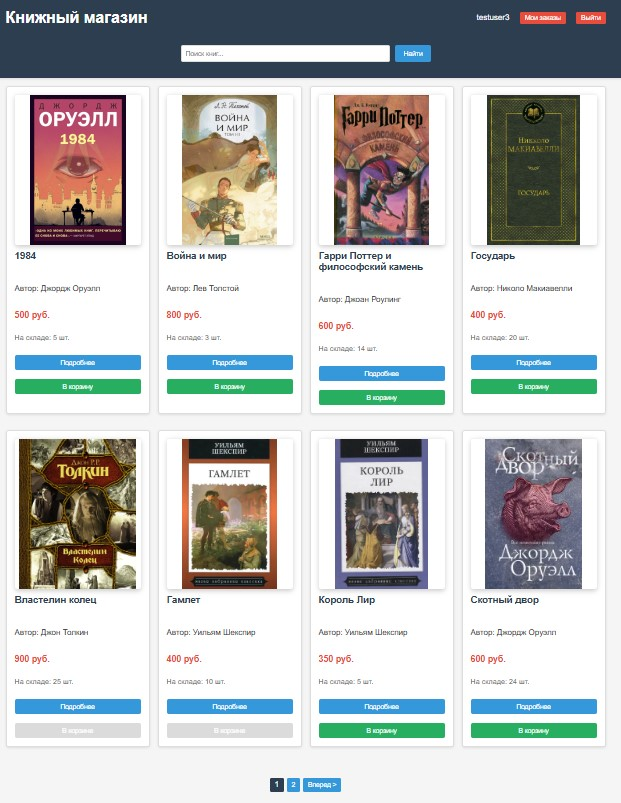
\includegraphics[width=0.9\linewidth]{images/Главная_страница_1}
	\caption{Главная страница сайта}
	\label{fig:1}
\end{figure}

На рисунке~\ref{fig:screenshot3} показано окно входа, обеспечивающее авторизацию пользователей. Модальное окно содержит поля для ввода имени пользователя и пароля, а также кнопку переключения на форму регистрации.
\begin{figure}[H]
	\centering
	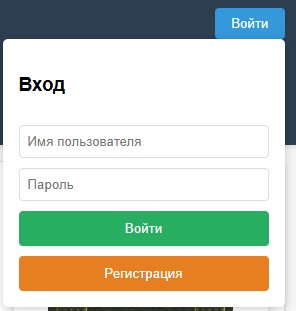
\includegraphics[width=0.5\linewidth]{images/Screenshot_3}
	\caption{Окно входа}
	\label{fig:screenshot3}
\end{figure}

На рисунке~\ref{fig:book_details} представлена подробная информация о книге, отображаемая в модальном окне при выборе книги из каталога. Окно включает название, автора, цену, дату публикации, жанры, описание и наличие на складе, а также кнопку добавления в корзину, что демонстрирует корректную работу функции просмотра деталей.
\begin{figure}[H]
	\centering
	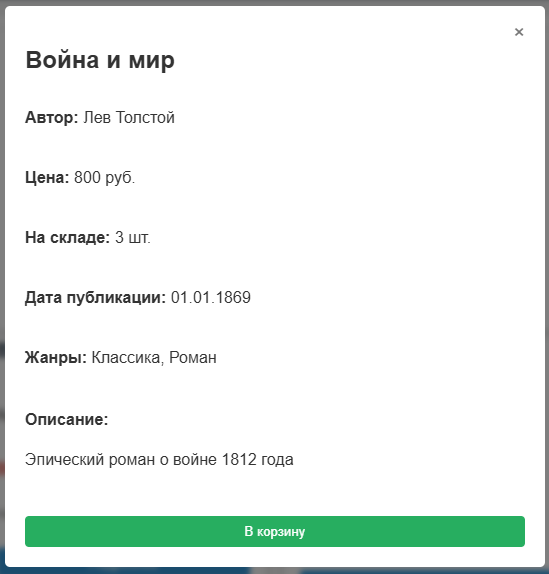
\includegraphics[width=0.7\linewidth]{images/подробнее}
	\caption{Подробная информация о книге}
	\label{fig:book_details}
\end{figure}

На рисунке~\ref{fig:screenshot5} продемонстрирована работа поисковой строки, позволяющая фильтровать книги по названию.
\begin{figure}[H]
	\centering
	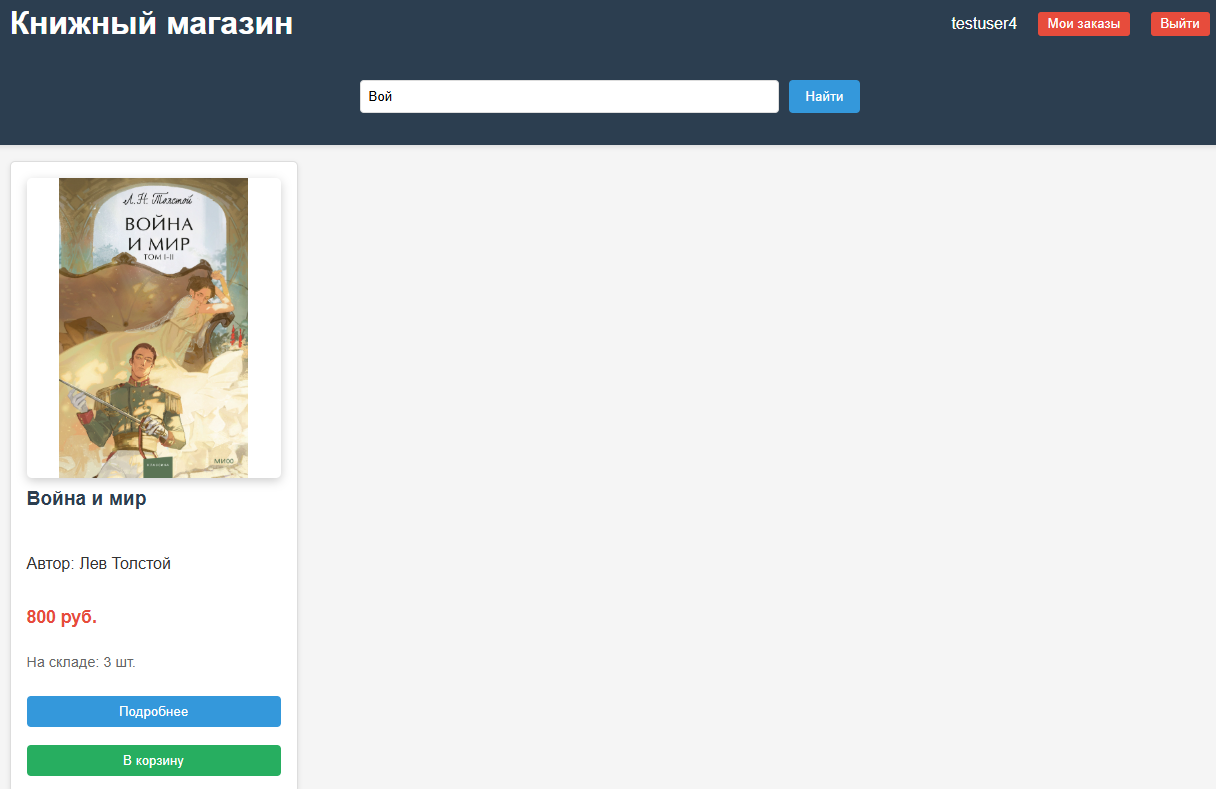
\includegraphics[width=0.8\linewidth]{images/Screenshot_5}
	\caption{Демонстрация работы поисковой строки}
	\label{fig:screenshot5}
\end{figure}

На рисунке~\ref{fig:cart} изображена корзина пользователя, содержащая выбранные книги с возможностью изменения количества и удаления позиций. Итоговая сумма обновляется автоматически, а кнопка «Оформить заказ» активна при наличии товаров.
\begin{figure}[H]
	\centering
	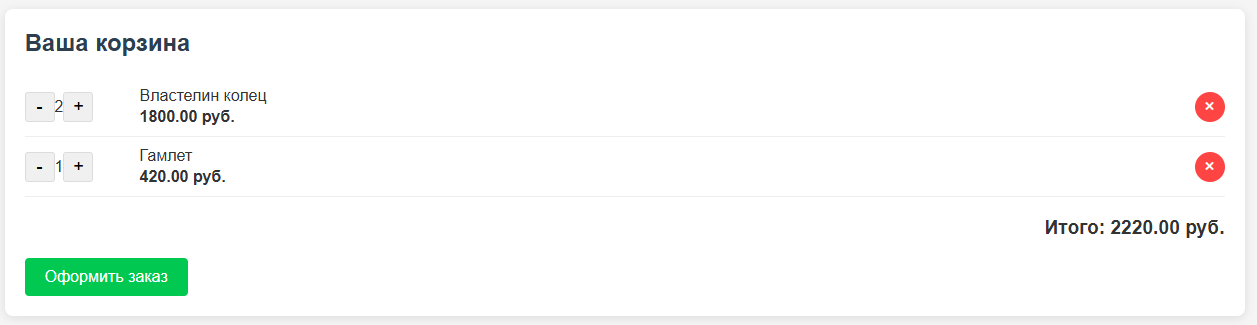
\includegraphics[width=0.9\linewidth]{images/корзинка}
	\caption{Корзина пользователя}
	\label{fig:cart}
\end{figure}

На рисунке~\ref{fig:order_success} показано уведомление об успешном оформлении заказа с указанием номера, даты, суммы и статуса.
\begin{figure}[H]
	\centering
	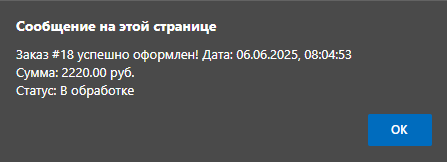
\includegraphics[width=0.7\linewidth]{images/заказсделан}
	\caption{Уведомление об успешном заказе}
	\label{fig:order_success}
\end{figure}

На рисунке~\ref{fig:222} представлен список заказов пользователя, включающий книги, номер, дату, сумму и статус.
\begin{figure}[H]
	\centering
	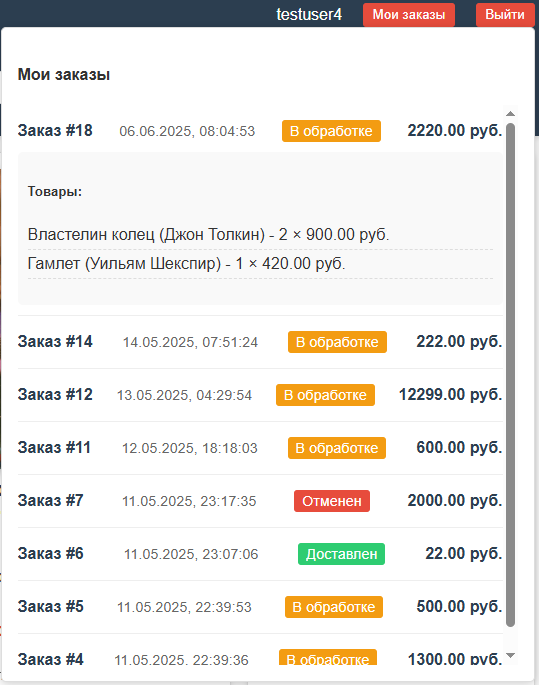
\includegraphics[width=0.7\linewidth]{images/222}
	\caption{Список заказов пользователя}
	\label{fig:222}
\end{figure}

На рисунках~\ref{fig:22},~\ref{fig:33},~\ref{fig:44},~\ref{fig:55} и~\ref{fig:66} показана главная страница, окно заказов и панель для пользователей с ролью администратора или сотрудника, предоставляющая доступ к функциям управления магазином. Интерфейс включает кнопки и панели для добавления и редактирования книг, а также просмотра заказов.
\begin{figure}[H]
	\centering
	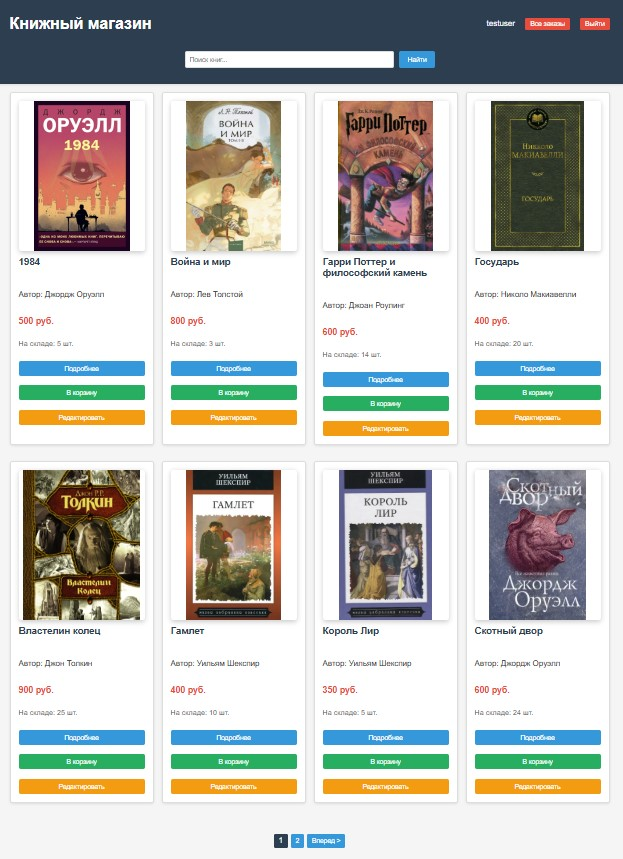
\includegraphics[width=0.9\linewidth]{images/Главная_страница_администратора}
	\caption{Главная страница администратора/сотрудника}
	\label{fig:22}
\end{figure}


\begin{figure}[H]
	\centering
	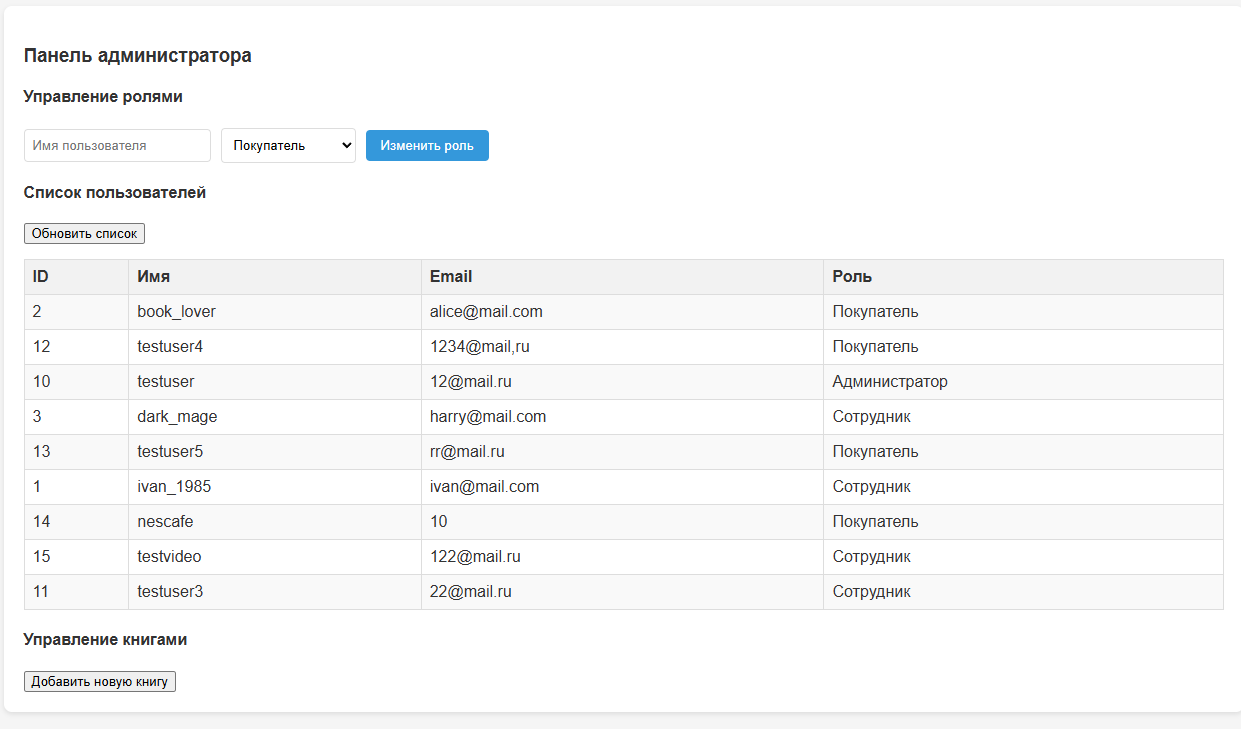
\includegraphics[width=0.9\linewidth]{images/панельадмина}
	\caption{Панель администратора}
	\label{fig:33}
\end{figure}

\begin{figure}[H]
	\centering
	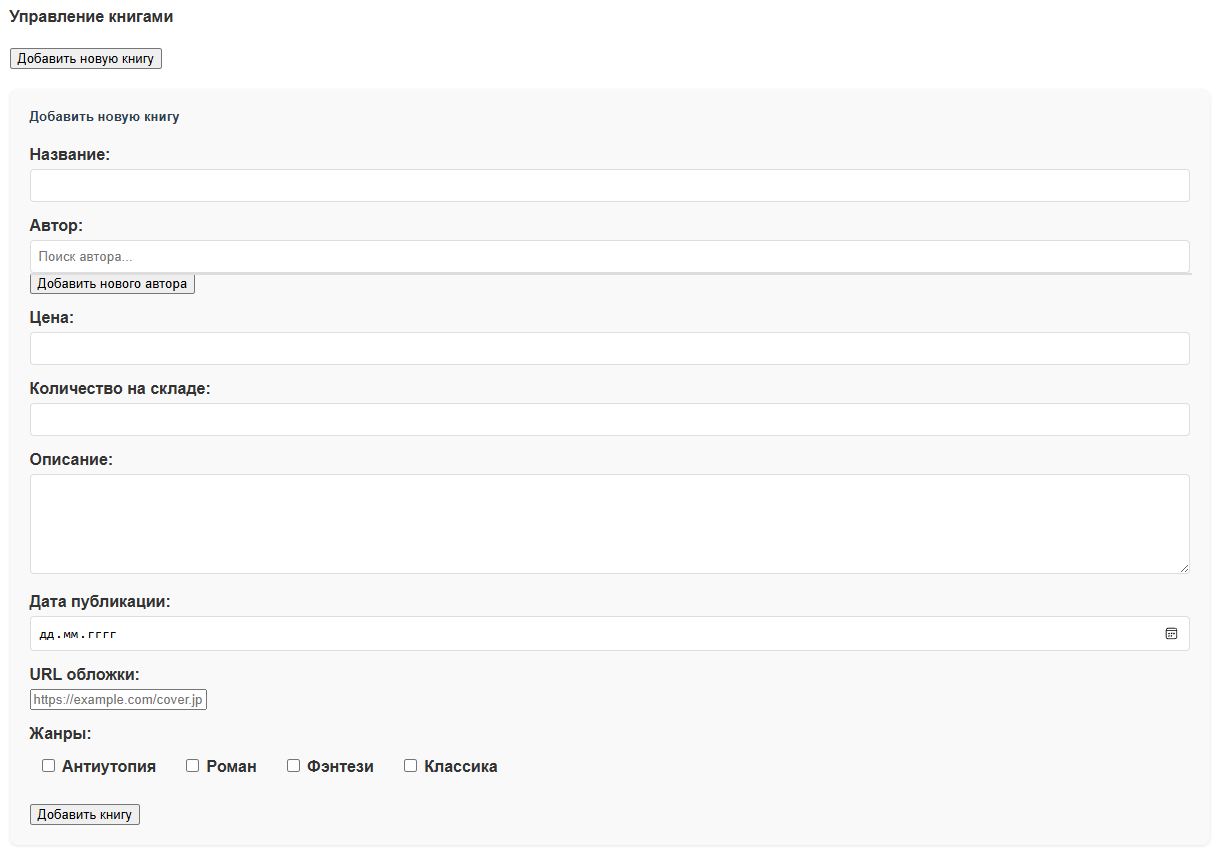
\includegraphics[width=0.9\linewidth]{images/добавление}
	\caption{Панель добавления новой книги}
	\label{fig:44}
\end{figure}

\begin{figure}[H]
	\centering
	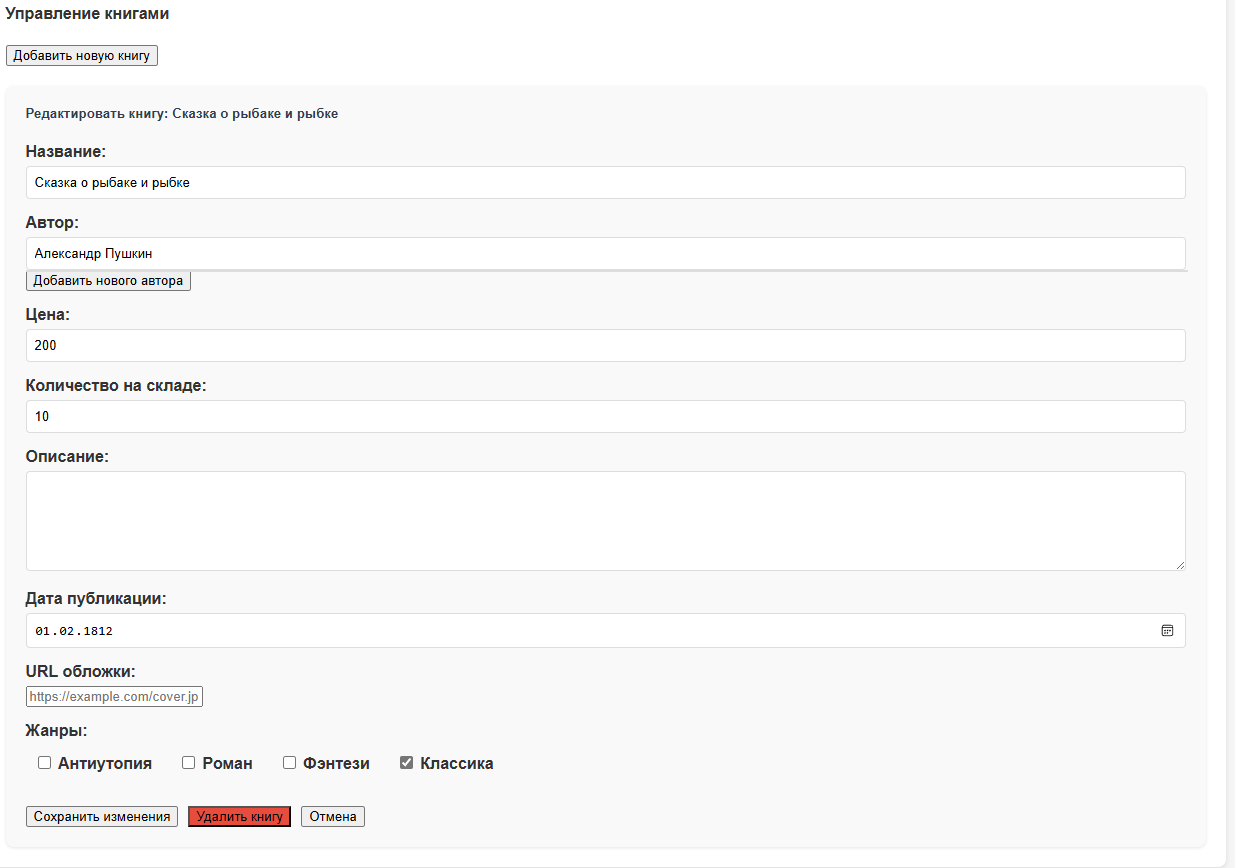
\includegraphics[width=0.9\linewidth]{images/редактирование}
	\caption{Панель редактирования существующей книги}
	\label{fig:55}
\end{figure}

\begin{figure}[H]
	\centering
	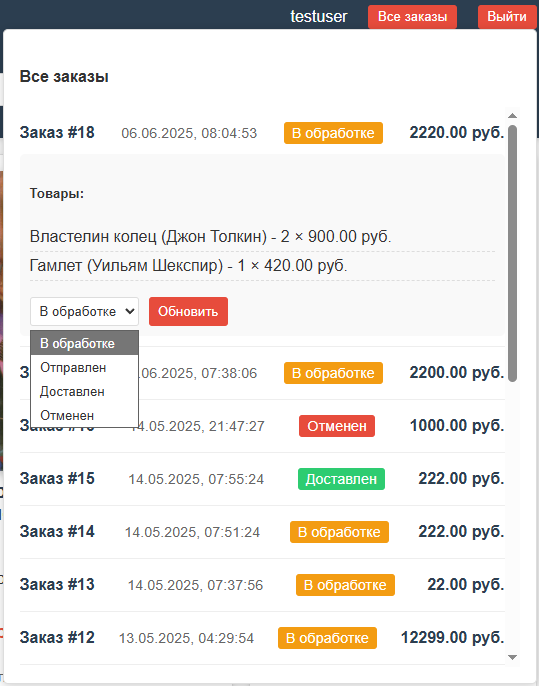
\includegraphics[width=0.9\linewidth]{images/админзаказы}
	\caption{Окно управления заказами всех пользователей}
	\label{fig:66}
\end{figure}

\subsection{Сборка программной системы}
Программные компоненты включают файлы исходного кода: app.py, app.js, index.html и styles.css.

Для сборки серверной части использовалась библиотека PyInstaller, которая упаковывает Python-код и зависимости в один исполняемый файл .exe. Этот файл запускается без установки Python и библиотек.

Клиентская часть не требует компиляции и работает в браузере. Файлы размещаются в статической директории сервера Flask.

Интерпретация Python-кода выполняется встроенным интерпретатором в .exe-файле. Для базы данных PostgreSQL требуется отдельная установка.

Все компоненты собраны для запуска: сервер — как .exe в Windows, клиент — через браузер.